\section{Results \& Discussion}

The results of the three algorithms in this section are created on environment three.
They are illustrated using boxplots showing the execution time of 100 runs.


\paragraph{Fibonacci}
\begin{figure}[htbp]
	\centering
	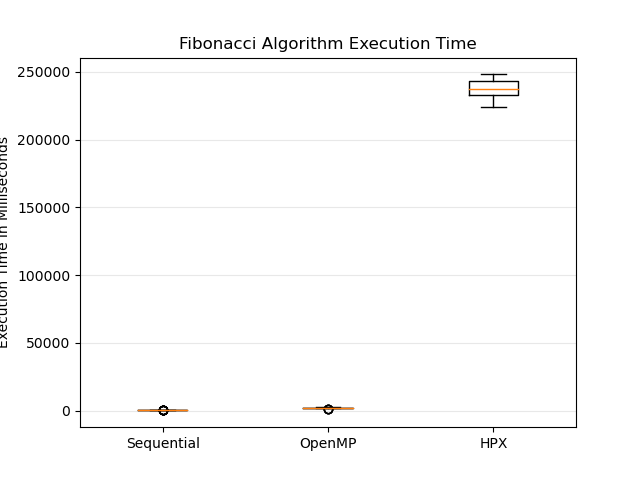
\includegraphics[width=0.45\textwidth]{figures/fib_NoOp.png}
	\caption{Execution Times of the Fibonacci Algorithm (Environment 3, 64 Threads)}
	\label{fig:fib_NoOp}
\end{figure}

Figure \ref{fig:fib_NoOp} shows the execution time of the 22\textsuperscript{nd} Fibonacci number.
It illustrates the times of the sequential, OpenMP and HPX version.
The sequential and OpenMP implementation need the fewest time to complete, whereas the HPX version takes a lot more time.

\paragraph{Merge Sort}
  \begin{figure}[htbp]
	\centering
	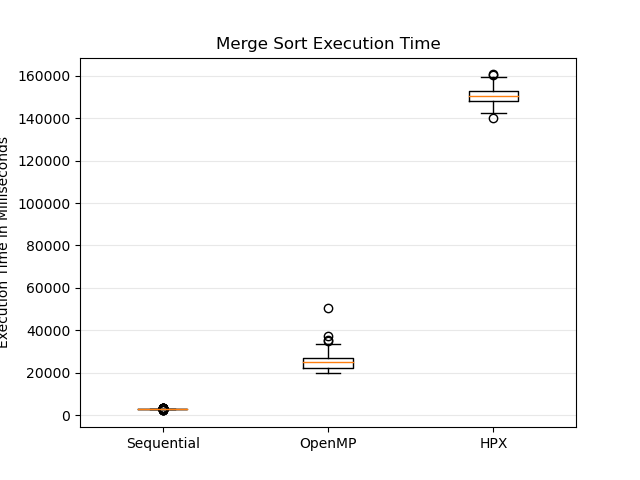
\includegraphics[width=0.45\textwidth]{figures/sort_NoOp.png}
	\caption{Execution times of Merge Sort (Environment 3, 64 Threads)}
	\label{fig:sort_NoOp}
  \end{figure}
  The measurements of figure \ref{fig:sort_NoOp} show the execution times of Merge Sort.
  The algorithm is run on 10.000 random elements which are created in a deterministic way.
  Similar to Fibonacci, merge sort also creates a lot of tasks and HPX shows the slowest execution time.
  Sequential has the shortest average time and the OpenMP average times differ more significantly this time compared to the Fibonacci example.
  
\paragraph{Generic Algorithm}
  \begin{figure}[htbp]
	\centering
	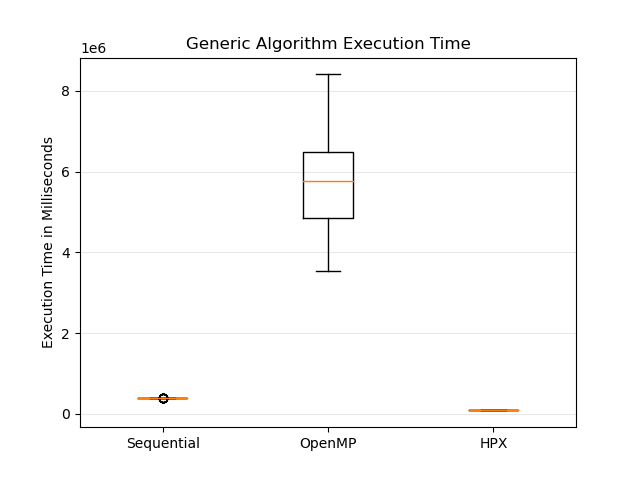
\includegraphics[width=0.45\textwidth]{figures/generic_NoOp.png}
	\caption{Execution times of the generic algorithm (Environment 3, 64 Threads)}
	\label{fig:gen_NoOp}
\end{figure}
Figure \ref{fig:gen_NoOp} shows the measured execution times for the generic algorithm in his three versions.
20 turns are made with a task size of 20 and the array size is 1,048,576.
It can be seen that the range of OpenMP times is quite big compared to the sequential and HPX version.
Additionally, the OpenMP version takes the longest time to complete the execution whereas HPX is the fastest of these three. 

\subsection{Discussion}
It can be seen that HPX has some issues keeping up with the sequential and OpenMP implementation of Fibonacci and Merge Sort.
Both algorithms spawn a lot of tasks in hierarchical structure.
This means each task, except of the root task, has a parent task.
This parent task has to suspend its execution until its child tasks finished their execution.
In contrast to threads in OpenMP HPX threads may be suspended which results in scheduling tasks occurring more often.
This leads to a bigger scheduling workload for HPX.

The generic algorithm however uses a different structure as it spawns various tasks for an array which need to be finished before spawning the next tasks for the next turn.
In this concept HPX can use its strength of lightweight threads.
These fork and join faster and with less work to do.

